\chapter{Materials and methods}
\section{Data Sets}

In this thesis, I will experiment with data sets where one class is significantly less than the other.
There are four datasets that I actually experimented with.
The first one I used was a simple dataset. This is a two-dimensional data set that can be easily visualized.
First, I will focus on visualizing and understanding the data.
Next, I will use a real data set. I use the UCI Machine Learning Repository\cite{UCI} for the data.

The actual data used were four.
We used four datasets: German Credit Dataset, HabermanDataset, Census-Income (KDD) Dataset, and Blood Transfusion Service Center Dataset.
The specifics of the datasets are described below.

\subsection{Simple 2D Data Set}
Create a random two-class classification problem.
It was generated using scikit-learn datasets make classification
The number of samples is set to 10000, The number of informative features is two,
The number of clusters per class is two, the ratio of classes is biased 99 to 1, and the clusters are put on the vertices of a hypercube.

For actual visualization, see Fig. 2.1.
\begin{center}
    \begin{figure*}[ht]
        \caption{Simple two-dimensional data set visualization}
        \label{tab:team-rating-features}
        \begin{center}
            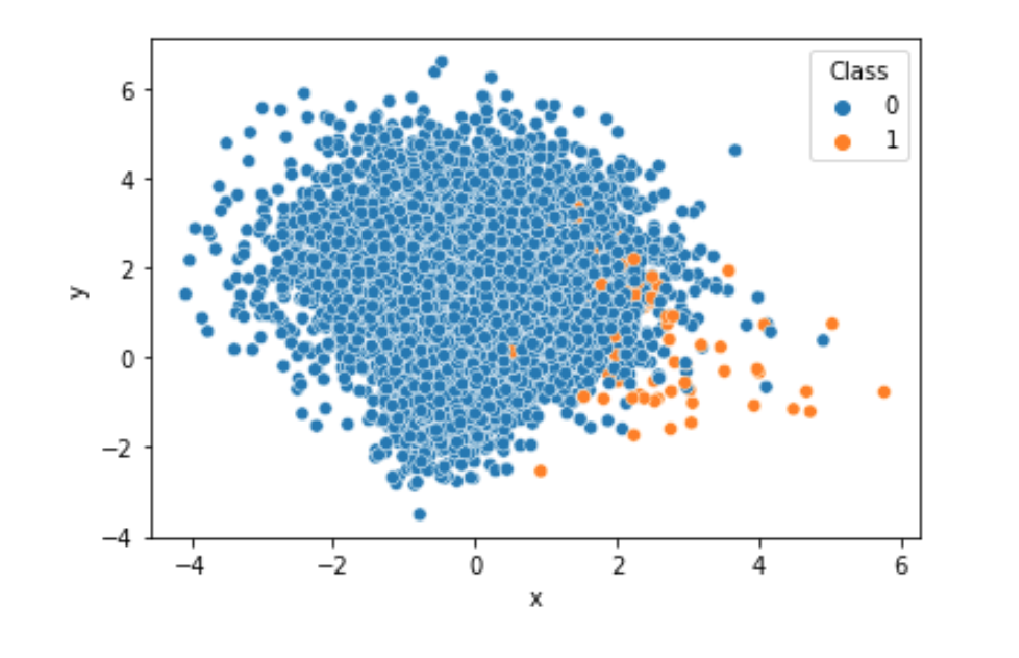
\includegraphics[scale=0.8]{image/data1.eps}
        \end{center}
    \end{figure*}
\end{center}

\subsection{German Credit Dataset}

The German Credit Dataset was downloaded from the UCI Machine Learning Repository, a web site that maintains many real datasets\cite{German}. 

The data set contains 1000 entries with 20 prepared category/symbol attributes
In this data set, each entry represents a person who receives credit from a bank. Each person is classified as a good or bad credit risk according to a set of attributes. We estimate it.
The data set is skewed with 700 out of 1000 entries for good credit risk.


\subsection{Haberman's Survival Data Set}

Haberman's Survival Data Set was similarly downloaded from the UCI Machine Learning Repository\cite{Haberman}.

The dataset contains case studies of survival of patients undergoing surgery for breast cancer conducted at the Billings Hospital of the University of Chicago between 1958 and 1970.
It has 306 data counts and three feature sets.
Estimate whether the patient died within 5 years.
It is a biased data set with 225 data that died within 5 years compared to 81 data that did not.

\subsection{Census-Income (KDD) Data Set}

The Census-Income (KDD) Data Set was similarly downloaded from the UCI Machine Learning Repository\cite{Census}.
This dataset contains weighted census data drawn from the 1994 and 1995 Current Population Surveys conducted by the U.S. Census Bureau. The data includes 41 demographic and employment related variables.
All categorical variables can be transformed into a Sparse One-Hot vector.
What we estimate is whether the income is greater than 50K or not.
We have a very large number of data, 32561, and the data is biased with 24720 being less than 50K.

\subsection{Blood Transfusion Service Center Data Set}

The Blood Transfusion Service Center Data Set was similarly downloaded from the UCI Machine Learning Repository\cite{Blood}.

This dataset contains data obtained from a blood transfusion service center located in Hsin Chu, Taiwan.
The center gives its blood transfusion service bus to one of the universities in Hsin Chu and collects donated blood about every three months. To build the FRMTC model, we randomly selected 748 donors from the donor database. For these 748 donor data, four variables were included. These are used to estimate whether a given donor has donated blood or not.

The data set is skewed, with 178 people who have donated blood compared to 570 who have not done so.
\clearpage


\section{Methods}
\subsection{SMOTE}

SMOTE is one method of random oversampling that increases the number of minority cases by randomly replicating the minority cases.

Below are the biased datasets.
Blue is the minority data set and orange is the majority data set.This can be seen in Fig. 2.2.

\begin{center}
    \begin{figure*}[ht]
        \caption{SMOTE: Before Oversampling.}
        \label{tab:team-rating-features}
        \begin{center}
            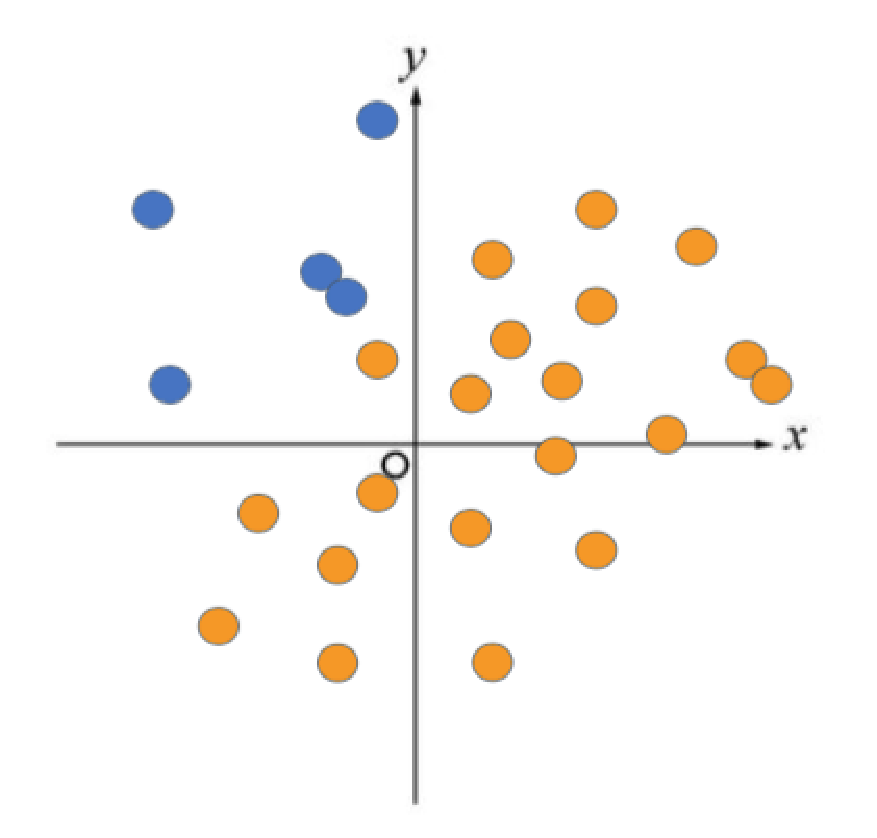
\includegraphics[scale=0.6]{image/smote1.eps}
        \end{center}
    \end{figure*}
\end{center}

\clearpage

Select one number group case. It's called $m_a$. This can be seen in Fig. 2.3.

\begin{center}
    \begin{figure*}[ht]
        \caption{SMOTE: Select a Case.}
        \label{tab:team-rating-features}
        \begin{center}
            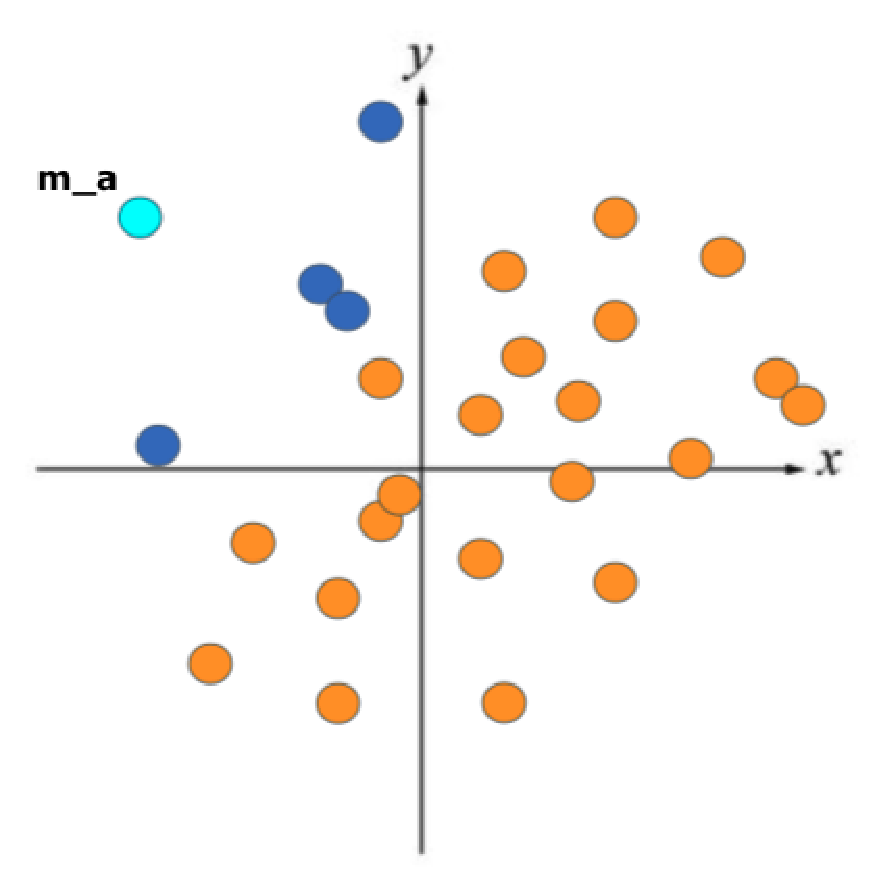
\includegraphics[scale=0.6]{image/smote2.eps}
        \end{center}
    \end{figure*}
\end{center}

\clearpage

Extract k data using the k-nearest neighbor method.
Calculate the degree of similarity between cases for a set of values of explanatory variables.
The similarity between vectors is calculated using the Euclidean distance

The j-th elements of $m_a$ and $m_i$ are written as $a_j$ and $i_j$, respectively.
$$
dis(m_a, m_i) = \Sigma_j(a_j - i_j)^2
$$
The figure below shows the k nearest neighbors painted in green. Figs2.4

\begin{center}
    \begin{figure*}[ht]
        \caption{SMOTE: Shows k nearest neighbor.}
        \label{tab:team-rating-features}
        \begin{center}
            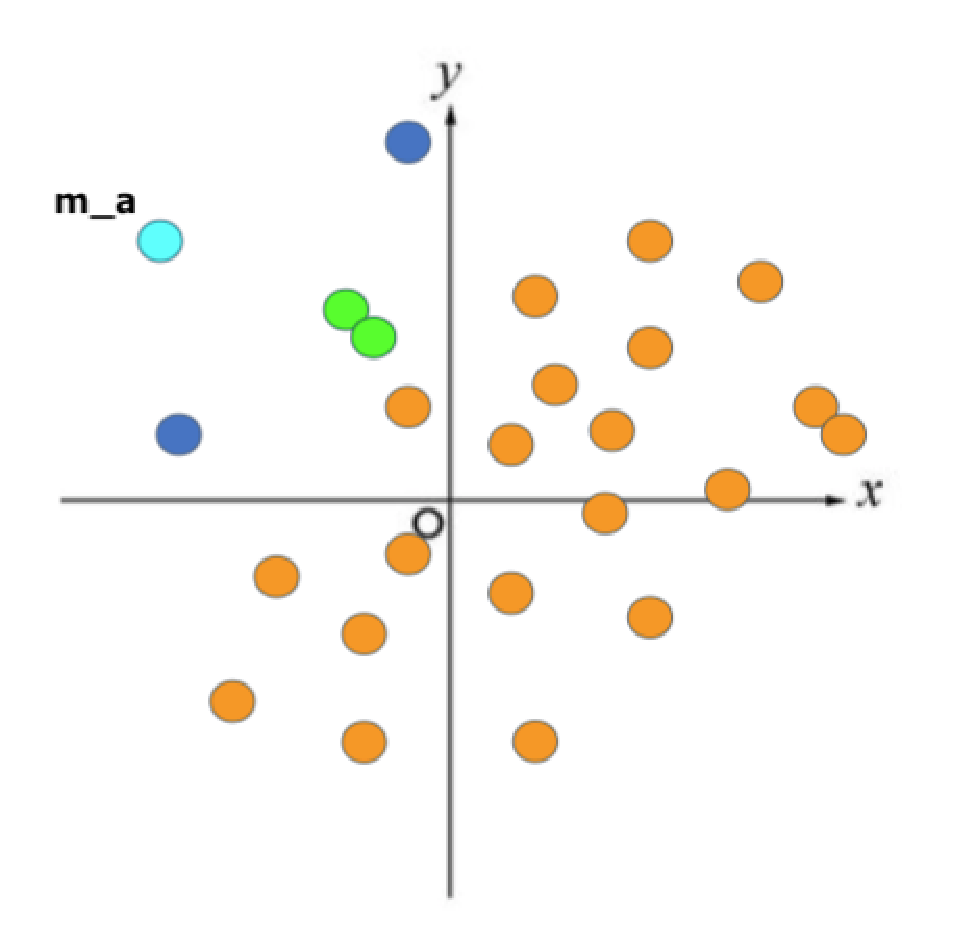
\includegraphics[scale=0.6]{image/smote3.eps}
        \end{center}
    \end{figure*}
\end{center}

\clearpage

Randomly select one of the k nearest neighbors.
In other words, pick one of the data that is colored green. Randomly.
I painted the selected one yellow.Figs2.5

\begin{center}
    \begin{figure*}[ht]
        \caption{SMOTE: Choose One Case from k nearest neighbors.}
        \label{tab:team-rating-features}
        \begin{center}
            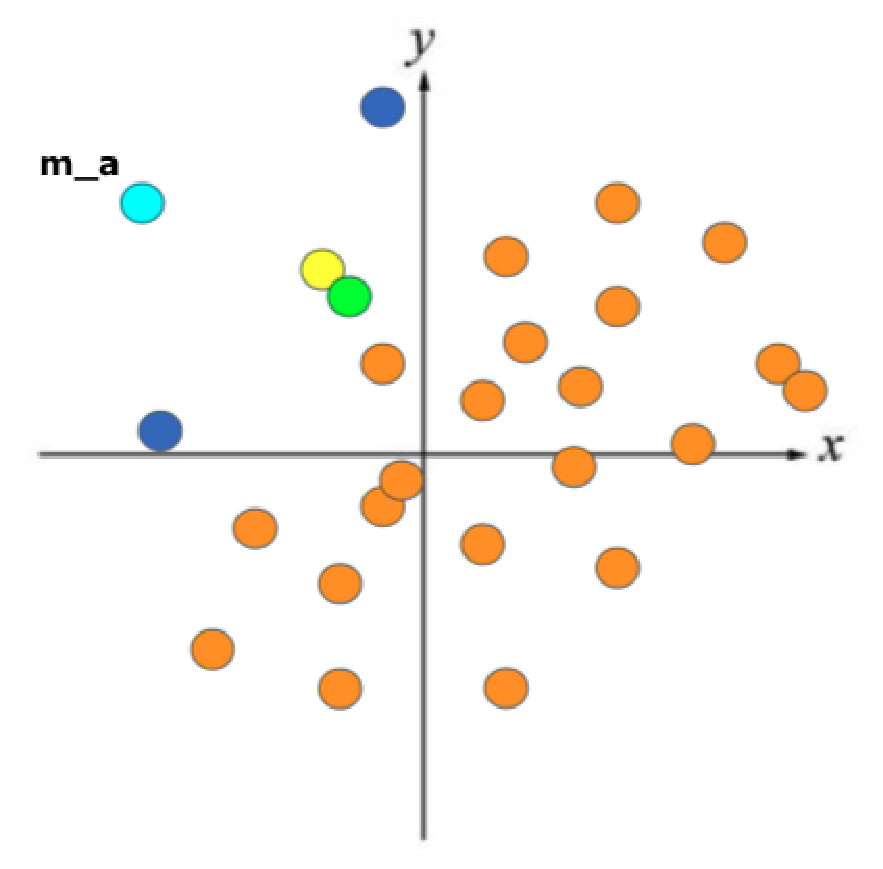
\includegraphics[scale=0.6]{image/smote4.eps}
        \end{center}
    \end{figure*}
\end{center}

\clearpage
Connect the first data you selected with the data you just selected with a straight line. Figs2.6.

\begin{center}
    \begin{figure*}[ht]
        \caption{SMOTE: Increase the number of new data in a linear fashion.}
        \label{tab:team-rating-features}
        \begin{center}
            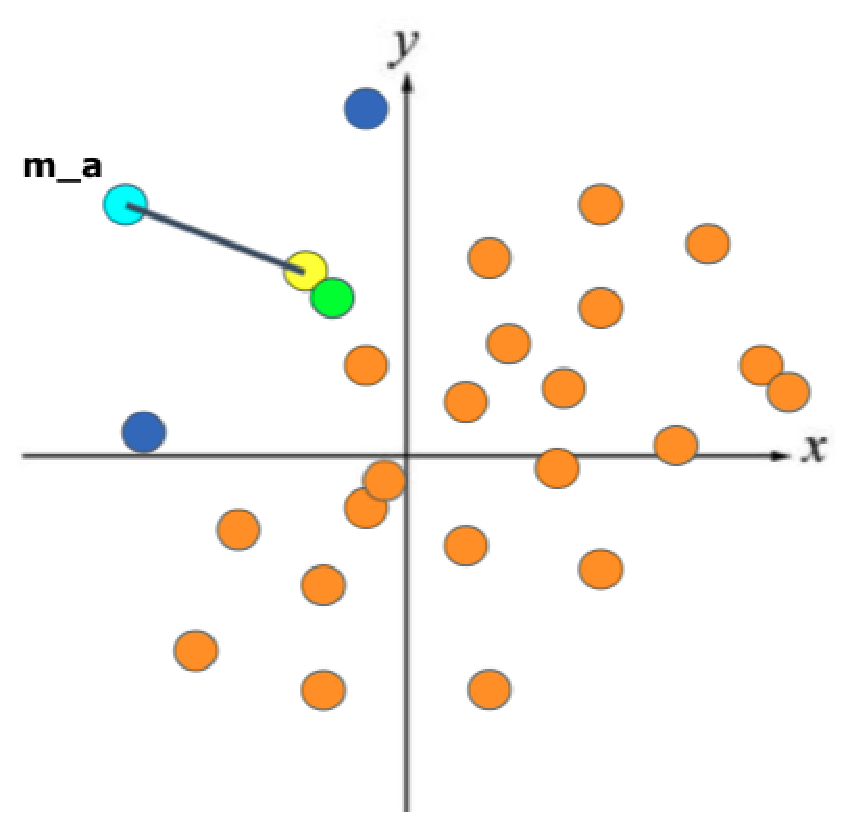
\includegraphics[scale=0.6]{image/smote5.eps}
        \end{center}
    \end{figure*}
\end{center}

It then generates some new data on that line.
This is the data that is generated by oversampling.
The position of the data on the line is completely random.

\clearpage
\subsection{Tomek-links}

One method of undersampling, which removes noisy samples, is to reduce the majority of the data set from a combination called Tomek Links.

The algorithm is described below.
Below is a biased data set.
Blue is the minority data set and orange is the majority data set.

\begin{center}
    \begin{figure*}[ht]
        \caption{TOMEK-LINKS: Before undersampling dataset.}
        \label{tab:team-rating-features}
        \begin{center}
            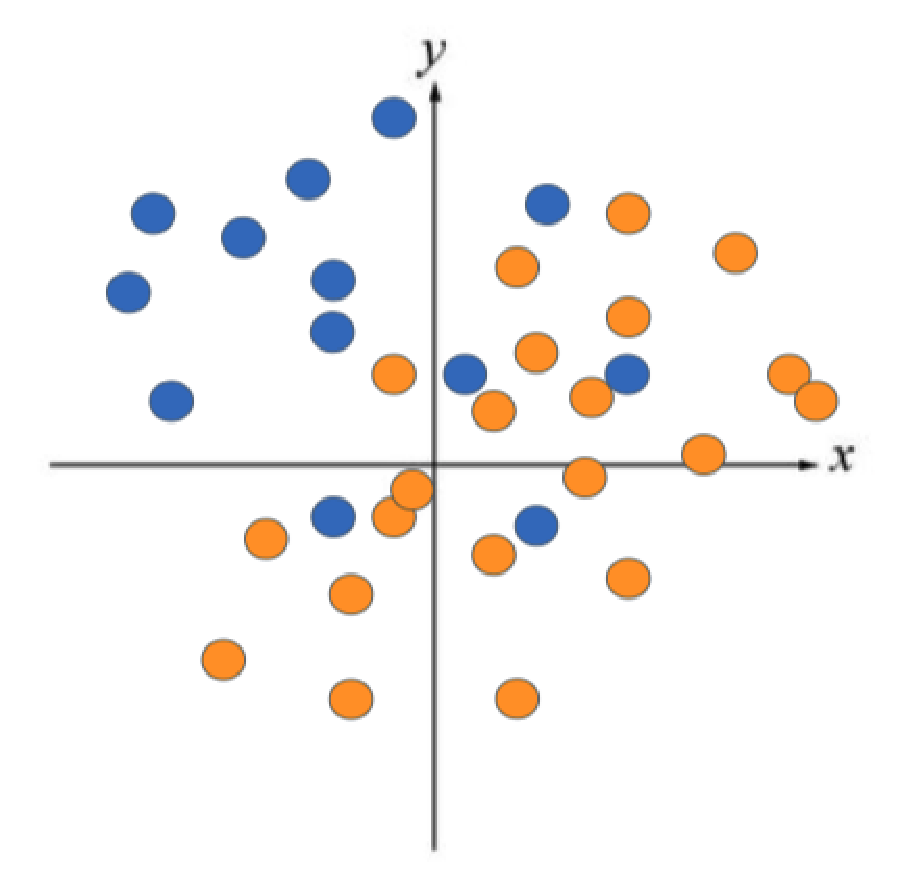
\includegraphics[scale=0.6]{image/tomek1.eps}
        \end{center}
    \end{figure*}
\end{center}

\clearpage

Tomek links are pairs of x and y such that there is no case z in the dataset that satisfies δ(x, z) < δ(x, y) or δ(y, z) < δ(y, x).
However, we define δ(x, y) to be the distance between the minority case x and the majority case y.

\begin{center}
    \begin{figure*}[ht]
        \caption{TOMEK-LINKS: Show the tomek-links.}
        \label{tab:team-rating-features}
        \begin{center}
            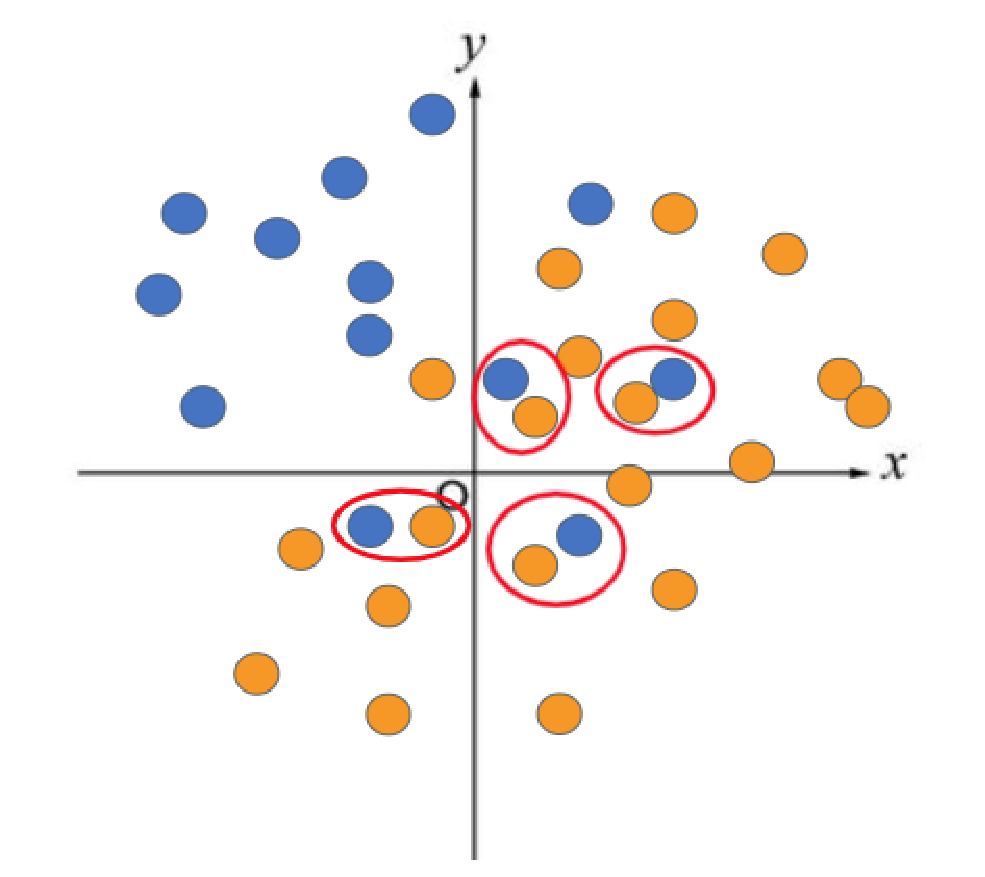
\includegraphics[scale=0.6]{image/tomek2.eps}
        \end{center}
    \end{figure*}
\end{center}

\clearpage

Delete the majority of data from these tomek links.

\begin{center}
    \begin{figure*}[ht]
        \caption{TOMEK-LINKS: Deleted tomek-links.}
        \label{tab:team-rating-features}
        \begin{center}
            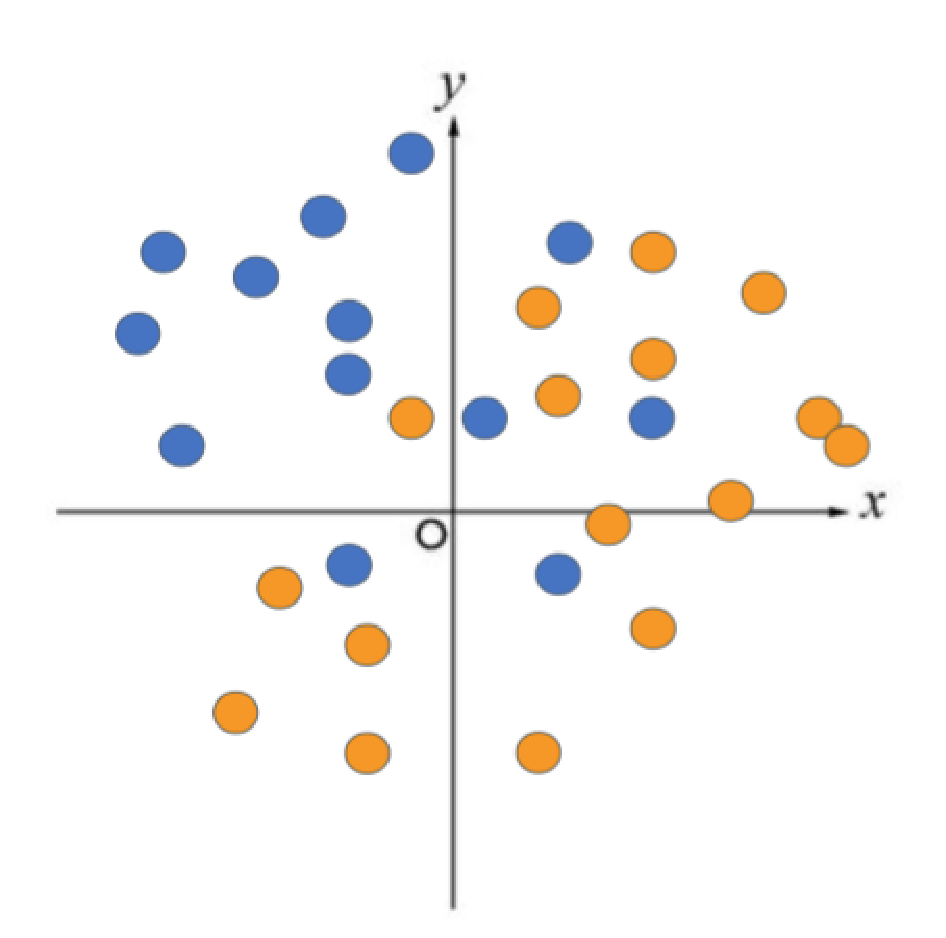
\includegraphics[scale=0.6]{image/tomek3.eps}
        \end{center}
    \end{figure*}
\end{center}

This process is repeated many times.

By repeating this process, we avoid having the majority of the data near the boundary, where the inferred value is obtained by violence of numbers.

\clearpage

\subsection{SMOTE + Tomek Combine}
In SMOTE + Tomek Combine, SMOTE and Tomek links are combined and over- and under-sampled.

\subsection{MySMOTE}

MySMOTE is an improved version of SMOTE.

Using a traditional smote produces a linear data set.
The boundaries between each class become blurred.
Change the algorithm for actually adding the data set.

For this reason, MySMOTE has devised a way to generate new data.

\begin{center}
    \begin{figure*}[ht]
        \caption{MYSMOTE: How to calculate the noise.}
        \label{tab:team-rating-features}
        \begin{center}
            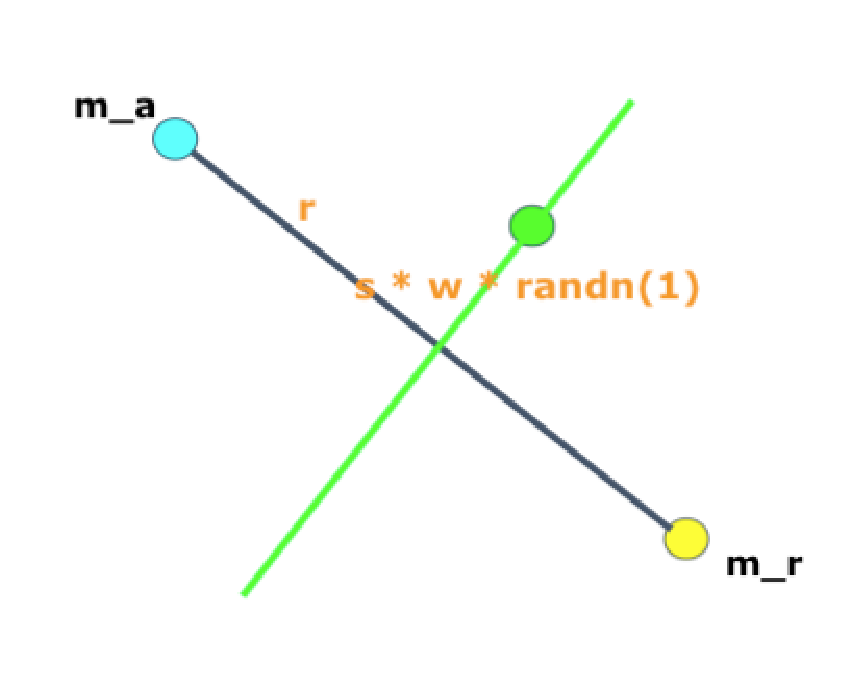
\includegraphics[scale=0.6]{image/mysmote1.eps}
        \end{center}
    \end{figure*}
\end{center}

Here is an explanation of the above variables.\\
r: This is a random value.
It is a ratio to a straight line and takes values from 0 to 1\\
s: Hyperparameter to determine how much noise to make.\\
w: This is the value of the variance of the explanatory variables.\\
I introduced it for the purpose of normalizing the magnitude of the noise to the explanatory variables.

